\chapter{Preliminaries}

\section{De Bruijn Graphs}

\subsection{Definition}

A \textbf{kmer} is a string of length $k$ over the alphabet $\Sigma$.

For $R$ a given set of strings over $\Sigma$, the representing \textbf{de Bruijn graph} of order $k$ is the directed graph $G = (V, E)$ where:
\begin{itemize}
    \item Each vertex corresponds to a unique kmer in $R$.
    \item There is a directed edge from vertex $u$ to vertex $v$ if and only if the suffix of $u$ of length $k-1$ is identical to the prefix of $v$ of length $k-1$
\end{itemize}

In genomic applications, the alphabet $\Sigma$ typically consists of the four nucleotides: $\Sigma = \{A, C, G, T\}$.

\begin{tikzpicture}[scale=1.5]
    % First row of nodes
    \node (A1) at (3, 2) {AGC};
    
    % Second row of nodes
    \node (B1) at (0, 0) {GCT};
    \node (B2) at (2, 0) {CTG};
    \node (B3) at (4, 0) {TGA};
    \node (B4) at (6, 0) {GAG};
    \node (B5) at (8, 0) {AGT};
    
    % Third row of nodes
    \node (C2) at (2, -2) {CTA};
    \node (C3) at (4, -2) {TAA};
    \node (C4) at (6, -2) {AAG};
    
    % Edges between nodes
    \draw[->] (B1) -- (B2);
    \draw[->] (B2) -- (B3);
    \draw[->] (B3) -- (B4);
    \draw[->] (B4) -- (B5);

    \draw[->] (B1) -- (C2);
    \draw[->] (C2) -- (C3);
    \draw[->] (C3) -- (C4);
    \draw[->] (C4) -- (B5);

    
    \draw[<-] (B1) -- (A1);
    \draw[<-] (A1) -- (B4);
  \end{tikzpicture}

\subsection{Compact de Bruijn Graphs}

\begin{tikzpicture}[scale=1.5]
    % First row of nodes
    \node (A1) at (2, 2) {AGC};
    
    % Second row of nodes
    \node (B1) at (0, 0) {GCT};
    \node (B2) at (2, 0) {CTGA};
    \node (B3) at (4, 0) {GAG};
    \node (B4) at (6, 0) {AGT};
    
    % Third row of nodes
    \node (C1) at (3, -2) {CTAAG};
    
    % Edges between nodes
    \draw[->] (B1) -- (B2);
    \draw[->] (B2) -- (B3);
    \draw[->] (B3) -- (B4);

    \draw[->] (B1) -- (C1);
    \draw[->] (C1) -- (B4);

    
    \draw[<-] (B1) -- (A1);
    \draw[<-] (A1) -- (B3);
  \end{tikzpicture}

\subsection{Colored de Bruijn Graphs}

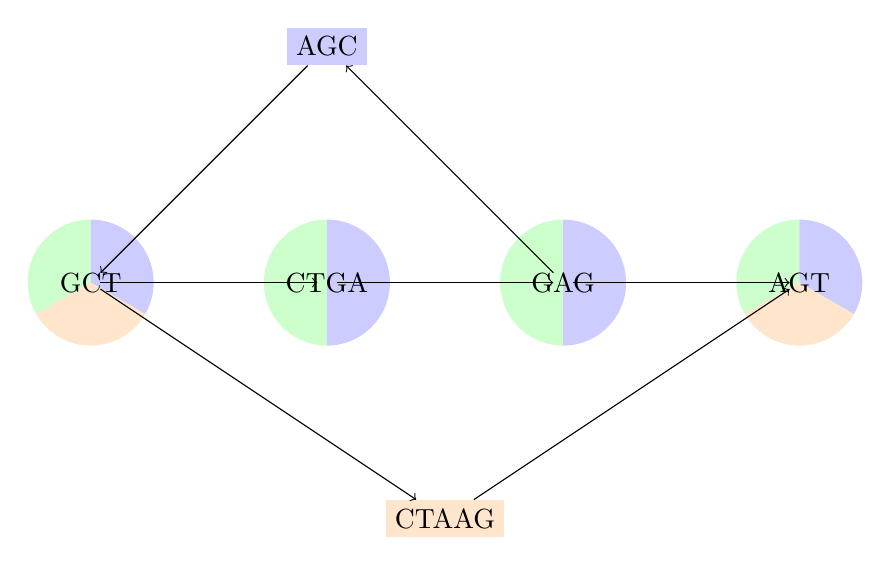
\begin{tikzpicture}[scale=1.5]
    % Define the size of the pic circles (note: pic and nodes are not the same)
    \def\a{1.6}
    % Style definitions for each row
    \tikzset{
        % one color
        one color/.style={fill=#1},
        % two colors
        pics/two colors/.style args=
        {#1|#2|label=#3}{code={%
            \fill[#1] (0,\a/2) arc(90:270:\a/2)--cycle;
            \fill[#2] (0,\a/2) arc(90:-90:\a/2)--cycle;
            \path (0,0) node[label={center:#3}] () {};
        }},
        % three colors
        pics/three colors/.style args=
        {#1|#2|#3|label=#4}{code={%
            \fill[#1] (0,\a/2) arc(90:210:\a/2)--(0,0)--cycle;
            \fill[#2] (0,\a/2) arc(90:-30:\a/2)--(0,0)--cycle;
            \fill[#3] (210:\a/2) arc(210:330:\a/2)--(0,0)--cycle;
            \path (0,0) node[label={center:#4}] () {};
        }}
    }
    % First row of nodes
    \node[one color=blue!20] (A1) at (2, 2) {AGC};

    % Second row of nodes
    \pic (B1) at (0, 0) {three colors={green!20|blue!20|orange!20|label=GCT}};
    \pic (B2) at (2, 0) {two colors={green!20|blue!20|label=CTGA}};
    \pic (B3) at (4, 0) {two colors={green!20|blue!20|label=GAG}};
    \pic (B4) at (6, 0) {three colors={green!20|blue!20|orange!20|label=AGT}};

    % Third row of nodes
    \node[one color=orange!20] (C1) at (3, -2) {CTAAG};

    % Edges between nodes
    \draw[->] (B1) -- (B2);
    \draw[->] (B2) -- (B3);
    \draw[->] (B3) -- (B4);

    \draw[->] (B1) -- (C1);
    \draw[->] (C1) -- (B4);

    \draw[<-] (B1) -- (A1);
    \draw[<-] (A1) -- (B3);
\end{tikzpicture}


% \begin{figure}[htbp]
%     \centering
%     % Placeholder for a de Bruijn graph illustration
%     % \includegraphics[width=0.8\textwidth]{debruijn_graph_example.png}
%     \caption{Example of a de Bruijn graph constructed from short reads. (a) Original reads. (b) Extraction of $k$-mers ($k=3$). (c) Resulting de Bruijn graph where nodes are $(k-1)$-mers and edges represent $k$-mers. (d) A possible Eulerian path through the graph (highlighted) representing a candidate assembly.}
%     \label{fig:debruijn}
% \end{figure}